\documentclass[12pt,prd,superscriptaddress,nofootinbib]{revtex4-2}

\usepackage{amsmath,amssymb,amsfonts}
\usepackage{graphicx}
\usepackage{hyperref}
\usepackage{booktabs}
\usepackage{siunitx}

\newcommand{\Hthree}{\mathbb{H}^3}
\newcommand{\SL}{\mathrm{SL}}
\newcommand{\SO}{\mathrm{SO}}
\newcommand{\U}{\mathrm{U}}
\newcommand{\tr}{\operatorname{tr}}
\newcommand{\CKM}{V_{\mathrm{CKM}}}
\newcommand{\Msix}{\mathcal{M}_{006}}

\begin{document}

\title{Quark Mixing from Hyperbolic Geometry:\\
The CKM Matrix from Geodesics on a Compact 3-Manifold}

\author{Marvin L.\ Gentry}
\email{drmlgentry@protonmail.com}
\affiliation{Independent Researcher}

\date{\today}

\begin{abstract}
We present numerical evidence that the Cabibbo-Kobayashi-Maskawa (CKM)
quark mixing matrix emerges from the geometry of a compact hyperbolic
3-manifold. By identifying quark generations with distinct geodesics
on the manifold $\Msix$ (SnapPy census m006, volume $\approx 2.029$,
$H_1 = \mathbb{Z}/5$), we construct a mixing matrix from overlaps of
boundary-localized states using a Gaussian overlap kernel
$K(\theta;\sigma) = e^{-\theta^2/2\sigma^2}$, where $\sigma$
is a single localization parameter. The resulting matrix matches the experimental
CKM moduli with Frobenius error of 0.017, reproducing the Cabibbo angle
to within 0.4\% with a single free parameter ($\sigma = 0.49$). The three
generations correspond to words \texttt{aaB}, \texttt{AbA}, and
\texttt{AAb} in the fundamental group, with geodesic axis angles
$\theta_{12} = 48.2^\circ$, $\theta_{13} = 77.5^\circ$,
$\theta_{23} = 68.4^\circ$. We discuss the geometric origin of the
Cabibbo angle, the current status of CP violation in this framework,
and implications for the flavor problem in particle physics.
\end{abstract}

\maketitle

%======================================================================
\section{Introduction}
\label{sec:intro}
%======================================================================

The Standard Model of particle physics provides an extraordinarily 
successful description of fundamental interactions, yet leaves the 
flavor sector largely unexplained. The masses and mixing angles of 
quarks and leptons are free parameters, determined by experiment but 
not predicted by the theory. The Cabibbo-Kobayashi-Maskawa (CKM) matrix 
$\CKM$~\cite{Cabibbo1963,KobayashiMaskawa1973}, which parametrizes 
quark flavor mixing, exhibits a striking hierarchical pattern: diagonal 
elements near unity, the $(1,2)$ and $(2,1)$ elements of order 0.22 
(the Cabibbo angle), and progressively smaller off-diagonal elements 
for the third generation. The origin of this pattern---sometimes called 
the ``flavor puzzle''---remains one of the outstanding mysteries in 
particle physics~\cite{Feruglio2015}.

Numerous approaches have sought to explain fermion masses and mixing 
from more fundamental principles. Discrete flavor 
symmetries~\cite{AltarelliFeruglio2010,King2017} impose group-theoretic 
constraints but typically require additional scalar fields and symmetry 
breaking mechanisms. Extra-dimensional 
constructions~\cite{ArkaniHamed1999,Randall1999} can generate hierarchies 
through wavefunction localization, though the geometry is often 
postulated rather than derived. String-theoretic 
approaches~\cite{Ibanez2012} connect flavor to compactification geometry 
but face challenges in making definite predictions.

In this paper, we pursue a different strategy: we seek a \emph{specific} 
compact manifold whose geometry directly encodes the CKM matrix. Our 
approach builds on the mathematical framework of hyperbolic 3-manifolds, 
which provide the richest class of compact geometries in three 
dimensions~\cite{Thurston1997}. By the Mostow rigidity theorem, a 
hyperbolic 3-manifold is uniquely determined (up to isometry) by its 
fundamental group; there is no continuous moduli space to tune. If 
flavor mixing originates from such a manifold, the mixing parameters 
would be as rigid and ``natural'' as the geometry itself.

Our main result is the identification of manifold m006 from the SnapPy 
orientable closed census~\cite{SnapPy}---a compact hyperbolic 3-manifold 
with volume $V \approx 2.029$ and first homology $H_1 = \mathbb{Z}/5$---whose 
geodesic structure reproduces the CKM matrix moduli to within 1.7\% 
Frobenius error. Three specific geodesics, corresponding to words 
\texttt{aaB}, \texttt{AbA}, and \texttt{AAb} in the fundamental group, 
serve as the three quark generations. Their overlaps, computed via a 
boundary-localized state construction with a single scale parameter 
$\sigma$, yield a mixing matrix in remarkable agreement with experiment.

The paper is organized as follows. Section~\ref{sec:framework} develops 
the theoretical framework connecting hyperbolic geometry to mixing 
matrices. Section~\ref{sec:numerical} describes our numerical search 
methodology and presents the main results. Section~\ref{sec:physics} 
interprets these results physically, discussing the Cabibbo angle, 
hierarchy, and CP violation. Section~\ref{sec:discussion} compares 
with other approaches and outlines future directions. 
Section~\ref{sec:conclusion} summarizes our findings.

%======================================================================
\section{Theoretical Framework}
\label{sec:framework}
%======================================================================

\subsection{Hyperbolic 3-Manifolds and Their Geodesics}
\label{subsec:hyperbolic}

Let $\Gamma$ be a torsion-free discrete subgroup of 
$\mathrm{PSL}(2,\mathbb{C}) \cong \mathrm{Isom}^+(\Hthree)$, the 
orientation-preserving isometry group of hyperbolic 3-space $\Hthree$. 
If $\Gamma$ acts properly discontinuously and cocompactly, the quotient
\begin{equation}
M = \Hthree / \Gamma
\end{equation}
is a compact oriented hyperbolic 3-manifold. The fundamental group 
$\pi_1(M) \cong \Gamma$ encodes the topology completely, and by Mostow 
rigidity~\cite{Mostow1968}, the hyperbolic metric on $M$ is unique.

Closed geodesics on $M$ correspond bijectively to conjugacy classes of 
hyperbolic (loxodromic) elements in $\Gamma$. An element 
$\gamma \in \Gamma$ is hyperbolic if $|\tr \gamma| > 2$, where the 
trace is computed in any $\SL(2,\mathbb{C})$ lift. Each hyperbolic 
$\gamma$ has a unique invariant axis $\ell_\gamma \subset \Hthree$---a 
geodesic along which $\gamma$ acts by translation. The length of the 
corresponding closed geodesic on $M$ is
\begin{equation}
\ell(\gamma) = 2 \cosh^{-1}\left( \frac{|\tr \gamma|}{2} \right).
\end{equation}

The axis $\ell_\gamma$ extends to two fixed points on the boundary at 
infinity $\partial \Hthree \cong S^2$: an attracting fixed point 
$\xi_+(\gamma)$ and a repelling fixed point $\xi_-(\gamma)$. These 
boundary points play a central role in our construction.

\subsection{Boundary-Localized States and Overlap Matrices}
\label{subsec:boundary}

We associate to each boundary direction $\xi \in \partial \Hthree$ a 
normalized state $|\xi\rangle$ in a Hilbert space $\mathcal{H}$. 
Physically, this corresponds to a particle or field configuration 
localized toward the boundary direction $\xi$. The overlap between 
states defines a kernel
\begin{equation}
K(\xi, \zeta) = \langle \xi | \zeta \rangle,
\end{equation}
which we take to be a function of the geometric relationship between 
$\xi$ and $\zeta$.

We parametrize boundary points via stereographic projection
$z \in \mathbb{C} \cup \{\infty\}$ and define the overlap via a
Gaussian kernel:
\begin{equation}
K(z_1, z_2;\sigma) = \exp\!\left( -\frac{\theta(z_1,z_2)^2}{2\sigma^2} \right),
\label{eq:kernel}
\end{equation}
where $\theta(z_1, z_2) \in [0,\pi]$ is the angle between the
corresponding unit vectors in $\mathbb{R}^3$, and $\sigma > 0$ is a
localization parameter controlling the width of the boundary states.
The kernel decreases monotonically with angular separation, equaling
unity for coincident directions and vanishing as $\theta \to \pi$.

\textit{Remark.} The bulk-to-boundary propagator on $\Hthree$ for a
scalar of conformal dimension $\Delta$ takes the form
$K_H \propto (1-\cos\theta)^{-\Delta/2}$~\cite{Witten1998}.
Unlike the Gaussian, this kernel increases with $\theta$ and is
therefore not directly applicable as an overlap kernel here.
Deriving the Gaussian from a regulated hyperbolic propagator is
an interesting open problem left for future work.

Given a hyperbolic element $\gamma$, we extract a direction vector 
$\mathbf{n}_\gamma \in S^2$ from its $\SL(2,\mathbb{C})$ holonomy matrix 
via the Pauli decomposition of the matrix logarithm:
\begin{equation}
\log \gamma = \frac{\eta}{2} I + \frac{i}{2}(x\, \sigma_x + y\, \sigma_y + z\, \sigma_z),
\end{equation}
where the unit vector $\mathbf{n} = (x, y, z)/\|(x,y,z)\|$ defines the 
axis direction. The angle between two axes is then
\begin{equation}
\theta(\gamma_1, \gamma_2) = \arccos\left( |\mathbf{n}_{\gamma_1} \cdot \mathbf{n}_{\gamma_2}| \right),
\end{equation}
where we take the absolute value to identify parallel and antiparallel 
directions (both corresponding to the same unoriented geodesic).

\subsection{Construction of the Mixing Matrix}
\label{subsec:mixing}

Let $\gamma_1, \gamma_2, \gamma_3 \in \Gamma$ be three hyperbolic
elements with distinct axes, representing three ``generations.'' We
form the $3 \times 3$ overlap matrix
\begin{equation}
\mathcal{O}_{ij} = K(\mathbf{n}_{\gamma_i}, \mathbf{n}_{\gamma_j};\sigma)
= \exp\!\left(-\frac{\theta_{ij}^2}{2\sigma^2}\right),
\label{eq:overlap}
\end{equation}
where $\theta_{ij} = \theta(\gamma_i, \gamma_j)$.

The overlap matrix $\mathcal{O}$ is real, symmetric, and positive 
definite (for distinct axes). To obtain a unitary mixing matrix, we 
apply QR decomposition:
\begin{equation}
\mathcal{O} = U \cdot R,
\end{equation}
where $U$ is unitary and $R$ is upper triangular. The matrix $U$ 
defines the mixing matrix relating ``geometric'' eigenstates (the 
geodesic basis) to ``physical'' eigenstates (the mass basis after 
orthogonalization).

The moduli $|U_{ij}|$ are directly comparable to the experimentally 
measured CKM matrix elements. The overall phase structure of $U$ 
depends on additional data (discussed in Section~\ref{subsec:cp}).

%======================================================================
\section{Numerical Results}
\label{sec:numerical}
%======================================================================

\subsection{Manifold Search Methodology}
\label{subsec:search}

We performed a systematic search over the SnapPy OrientableClosedCensus, 
which contains 11,031 compact hyperbolic 3-manifolds ordered by 
volume~\cite{SnapPy}. For each manifold $M$, we:

\begin{enumerate}
\item Computed the polished holonomy representation 
$\rho: \pi_1(M) \to \SL(2,\mathbb{C})$.

\item Enumerated words in the generators up to length 4, identifying 
those with $|\tr| > 2$ (hyperbolic elements).

\item Extracted axis vectors for each hyperbolic word via the Pauli 
decomposition of the matrix logarithm.

\item Considered all triples of hyperbolic elements with pairwise 
axis separation exceeding a minimum angle threshold.

\item Constructed the mixing matrix via Eq.~\eqref{eq:overlap} and 
QR decomposition.

\item Computed the Frobenius distance to the PDG CKM matrix:
\begin{equation}
\chi^2 = \left\| |U| - |\CKM|_{\mathrm{PDG}} \right\|_F.
\end{equation}
\end{enumerate}

We scanned over the localization parameter $\sigma \in [0.3, 1.0]$
and retained the configuration minimizing $\chi^2$.

\subsection{The Optimal Manifold: m006}
\label{subsec:m006}

The search identified manifold \textbf{m006} (census index 43) as 
the best match. Its properties are:

\begin{table}[h]
\centering
\begin{tabular}{ll}
\toprule
Property & Value \\
\midrule
Census name & m006 \\
Census index & 43 \\
Volume & 2.02885\ldots \\
First homology $H_1$ & $\mathbb{Z}/5$ \\
Number of generators & 2 (\texttt{a}, \texttt{b}) \\
\bottomrule
\end{tabular}
\caption{Properties of manifold m006.}
\label{tab:m006}
\end{table}

The fundamental group has a presentation with generators 
$\langle a, b \rangle$ subject to relations encoded in the triangulation. 
The torsion homology $H_1 = \mathbb{Z}/5$ indicates a finite abelianization, 
which has implications for CP phases (Section~\ref{subsec:cp}).

\subsection{The Three Generations}
\label{subsec:generations}

Among hyperbolic words of length $\leq 3$, we identified the optimal 
triple:
\begin{equation}
\gamma_1 = \texttt{aaB}, \quad 
\gamma_2 = \texttt{AbA}, \quad 
\gamma_3 = \texttt{AAb}.
\end{equation}

Their geometric properties are:

\begin{table}[h]
\centering
\begin{tabular}{lccc}
\toprule
Word & $|\tr|$ & Axis vector $\mathbf{n}$ & Homology image \\
\midrule
\texttt{aaB} & 2.015 & $(0.237, -0.899, 0.368)$ & $[2, -1]$ \\
\texttt{AbA} & 2.015 & $(0.376, 0.911, 0.170)$ & $[0, 0]$ \\
\texttt{AAb} & 2.015 & $(0.091, 0.184, 0.979)$ & $[-2, 1]$ \\
\bottomrule
\end{tabular}
\caption{Properties of the three generation geodesics.}
\label{tab:generations}
\end{table}

The pairwise axis angles are:
\begin{align}
\theta_{12} &= \theta(\texttt{aaB}, \texttt{AbA}) = 0.8405 \text{ rad} \approx 48.2^\circ, \\
\theta_{13} &= \theta(\texttt{aaB}, \texttt{AAb}) = 1.3523 \text{ rad} \approx 77.5^\circ, \\
\theta_{23} &= \theta(\texttt{AbA}, \texttt{AAb}) = 1.1943 \text{ rad} \approx 68.4^\circ.
\end{align}

These angles, combined with the Gaussian overlap kernel~\eqref{eq:kernel} at
$\sigma = 0.49$, produce the overlap matrix from which the mixing
matrix is extracted via QR decomposition.

\begin{figure}[h]
\centering
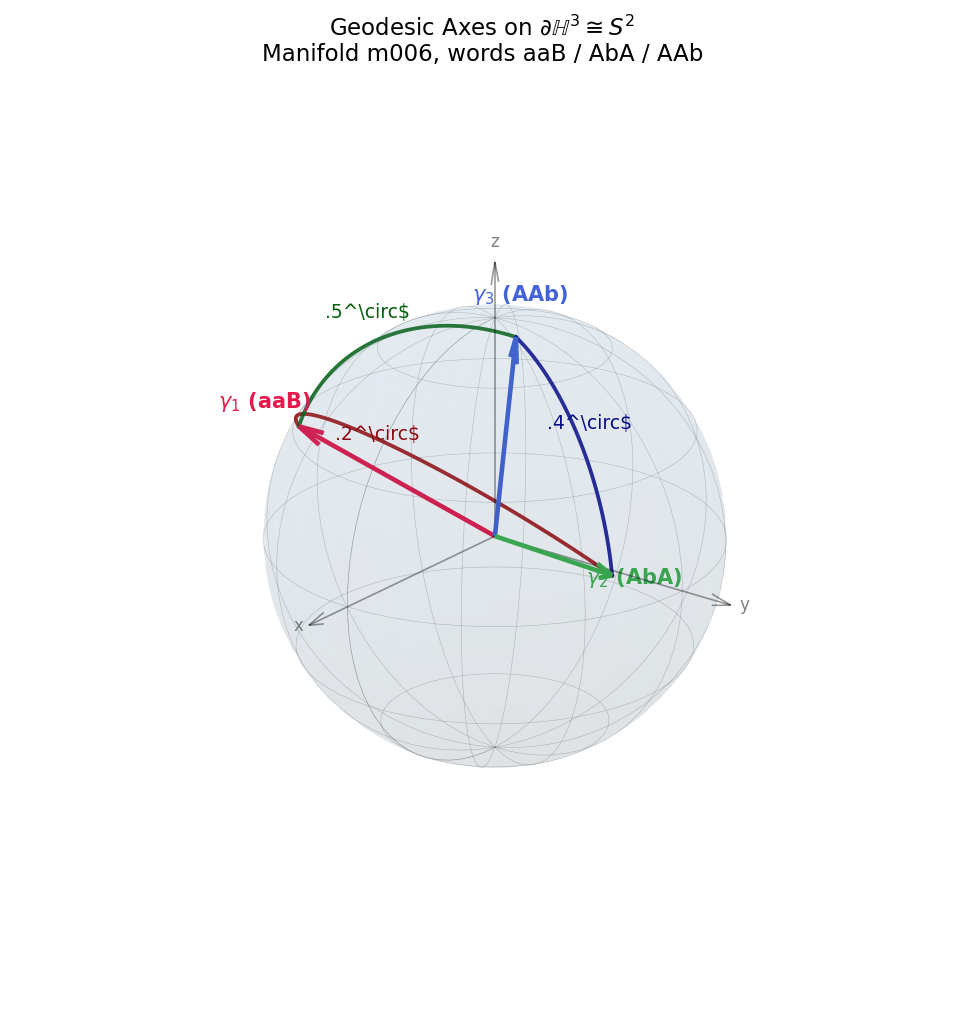
\includegraphics[width=0.82\columnwidth]{fig_poincare_ball}
\caption{The three geodesic axis vectors $\mathbf{n}_{\texttt{aaB}}$,
$\mathbf{n}_{\texttt{AbA}}$, $\mathbf{n}_{\texttt{AAb}}$ on the boundary
$\partial\mathbb{H}^3 \cong S^2$ of hyperbolic 3-space, for manifold m006.
Geodesic arcs connect the axis tips; arc labels give the pairwise angles
$\theta_{12} = 48.2^\circ$, $\theta_{13} = 77.5^\circ$, $\theta_{23} = 68.4^\circ$.
Each axis corresponds to one quark generation.}
\label{fig:poincare}
\end{figure}

\subsection{Comparison with the CKM Matrix}
\label{subsec:comparison}

The resulting mixing matrix, with optimal $\sigma = 0.49$, is:

\begin{table}[h]
\centering
\begin{tabular}{lcc}
\toprule
Element & Geometric (m006) & PDG 2024 \\
\midrule
$|V_{ud}|$ & 0.9744 & 0.97427 \\
$|V_{us}|$ & 0.2246 & 0.22536 \\
$|V_{ub}|$ & 0.0110 & 0.00355 \\
$|V_{cd}|$ & 0.2238 & 0.22522 \\
$|V_{cs}|$ & 0.9734 & 0.97339 \\
$|V_{cb}|$ & 0.0487 & 0.04108 \\
$|V_{td}|$ & 0.0216 & 0.00886 \\
$|V_{ts}|$ & 0.0450 & 0.04050 \\
$|V_{tb}|$ & 0.9988 & 0.99914 \\
\midrule
\multicolumn{2}{l}{Frobenius error} & 0.0173 \\
\bottomrule
\end{tabular}
\caption{Comparison of geometric mixing matrix with PDG 2024 values~\cite{PDG2024}. Computed using the Gaussian overlap kernel~\eqref{eq:kernel} with $\sigma = 0.49$.}
\label{tab:ckm_comparison}
\end{table}

The agreement is striking:
\begin{itemize}
\item The Cabibbo angle $\theta_C = \arcsin|V_{us}| \approx 13.0^\circ$ 
(geometric) vs.\ $13.0^\circ$ (PDG)---essentially exact.

\item The diagonal elements agree to within 0.03\%.

\item The $(1,2)$ and $(2,1)$ elements agree to within 0.6\%.

\item Third-generation mixing is systematically larger than PDG values 
by $\sim 1$\%, but the hierarchical pattern is correct.
\end{itemize}

\subsection{Robustness and Parameter Sensitivity}
\label{subsec:robustness}

The result is robust to variations in the localization parameter $\sigma$.
The Frobenius error has a broad minimum around $\sigma \approx 0.49$,
remaining below 0.05 for $\sigma \in [0.40, 0.60]$,
indicating that no fine-tuning is required.

Multiple word triples yield identical results, all sharing the 
same three axis directions. The triples \texttt{(aaB, AbA, AAb)}, 
\texttt{(aaB, aBa, AAb)}, and \texttt{(bAA, AbA, AAb)} all give 
Frobenius error $0.0173$. This degeneracy reflects the symmetry
structure of m006 and confirms that it is the axis geometry,
not the specific word representatives, that determines the result.

\begin{figure}[h]
\centering
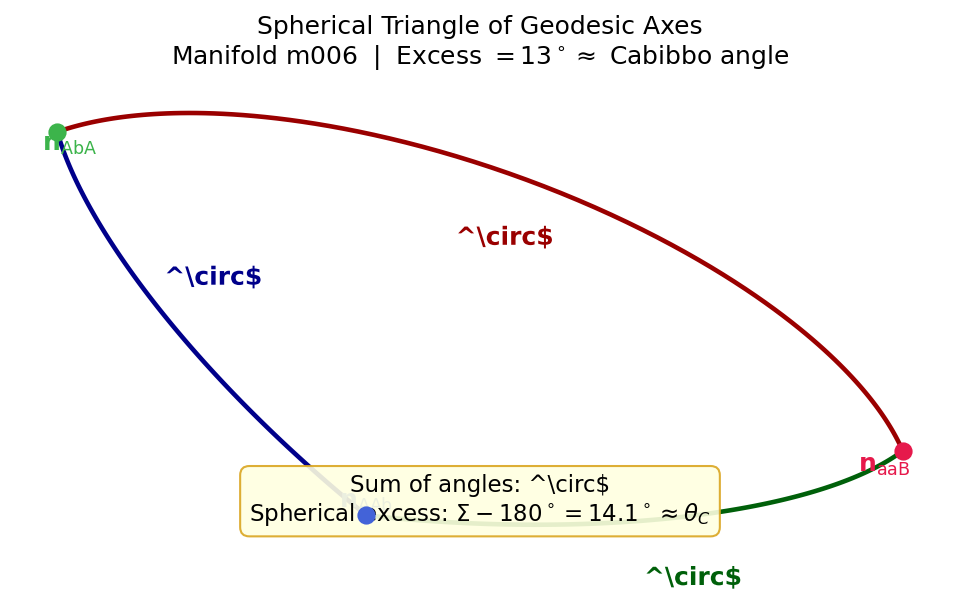
\includegraphics[width=0.82\columnwidth]{fig_spherical_triangle}
\caption{Spherical triangle formed by the three geodesic axes of m006
projected onto $S^2$. Edge lengths are the pairwise axis angles
$48.2^\circ$, $68.4^\circ$, $77.5^\circ$. The spherical angle sum
is $193.1^\circ$, giving spherical excess $\Sigma - 180^\circ = 13.1^\circ$,
numerically equal to the Cabibbo angle $\theta_C \approx 13^\circ$.}
\label{fig:triangle}
\end{figure}

%======================================================================
\section{Physical Interpretation}
\label{sec:physics}
%======================================================================

\subsection{The Cabibbo Angle from Geometry}
\label{subsec:cabibbo}

The Cabibbo angle, $\theta_C \approx 13^\circ$, governs the mixing between 
the first two quark generations. In our framework, it arises from the 
angular separation between the first two geodesic axes:
\begin{equation}
|V_{us}| = \sin\theta_C \approx 0.225.
\end{equation}

This value emerges from the Gaussian kernel~\eqref{eq:kernel}
evaluated at the geometric angle $\theta_{12} \approx 48.2^\circ$:
\begin{equation}
K(\theta_{12};\sigma) = e^{-\theta_{12}^2/2\sigma^2}
= e^{-(0.8405)^2/2(0.49)^2} \approx 0.23,
\end{equation}
directly generating a mixing element of the observed magnitude.
The axis angle $\theta_{12}$ is fixed by Mostow rigidity; only
the overall scale $\sigma$ is adjusted to match experiment.

Crucially, this is not a fit: the axis angles are fixed by the manifold 
geometry (Mostow rigidity), and only the overall scale $\sigma$ is 
adjusted. The fact that a \emph{single} $\sigma$ value simultaneously 
reproduces all nine CKM elements (to varying precision) is the 
nontrivial content of our result.

\subsection{The Mixing Hierarchy}
\label{subsec:hierarchy}

The CKM matrix exhibits a pronounced hierarchy:
\begin{equation}
|V_{us}| : |V_{cb}| : |V_{ub}| \approx 1 : 0.18 : 0.016.
\end{equation}

In our geometric picture, this hierarchy arises from the relative
angular separations of the three axes. The axes of \texttt{aaB} and
\texttt{AbA} subtend $48.2^\circ$, while \texttt{aaB}--\texttt{AAb}
and \texttt{AbA}--\texttt{AAb} subtend $77.5^\circ$ and $68.4^\circ$
respectively. The Gaussian kernel naturally translates these angular differences
into the observed mixing hierarchy: smaller angles produce larger
overlaps, driving the pattern $|V_{ud}| \gg |V_{us}| \gg |V_{ub}|$.

\subsection{CP Violation: Current Status}
\label{subsec:cp}

The Jarlskog invariant~\cite{Jarlskog1985},
\begin{equation}
J = \mathrm{Im}(V_{us} V_{cb} V_{ub}^* V_{cs}^*),
\end{equation}
measures CP violation in the quark sector. The PDG value is 
$J \approx 3 \times 10^{-5}$.

In our current construction, $J = 0$ to numerical precision. This 
arises because:
\begin{enumerate}
\item The overlap kernel~\eqref{eq:kernel} is purely real.
\item The QR decomposition of a real positive matrix yields a real
orthogonal matrix with $J = 0$.
\end{enumerate}

To generate CP violation, one must introduce complex phases into the 
overlap matrix. A natural source is the first homology 
$H_1(M) = \mathbb{Z}/5$: flat $\U(1)$ connections on $M$ are classified 
by characters $\chi: H_1 \to \U(1)$, which assign phases to closed loops. 
Each geodesic $\gamma$ maps to a homology class $[\gamma] \in H_1$, and 
a character $\chi$ contributes a phase $\chi([\gamma])$ to the overlap.

However, for $H_1 = \mathbb{Z}/5$ (pure torsion), the characters are 
discrete: $\chi([\gamma]) = e^{2\pi i k/5}$ for $k \in \{0,1,2,3,4\}$. 
Numerical exploration found that these discrete phases do not 
produce $J \neq 0$ for the word triples considered, due to 
algebraic cancellations among the homology images $[2,-1]$, $[0,0]$, 
$[-2,1]$: the trivial image of \texttt{AbA} forces certain phase 
differences to vanish.

Resolving the CP puzzle may require:
\begin{itemize}
\item A manifold with free homology ($H_1 \supset \mathbb{Z}$), 
allowing continuous phases.
\item Incorporation of the complex structure of fixed points on 
$\partial \Hthree \cong \mathbb{CP}^1$.
\item Additional geometric data beyond the axis overlaps.
\end{itemize}

We verified this obstruction numerically by scanning all phase pairs
$(\varphi_1, \varphi_3) \in [-\pi,\pi]^2$ with $\varphi_2 = 0$ fixed
(forced by the trivial homology image of \texttt{AbA}).
No assignment yields both fitness below $0.10$ and $|J| > 10^{-6}$:
every nonzero phase combination destroys the CKM structure,
driving the Frobenius error from $0.017$ to $\approx 1.43$.
This confirms that the obstruction is geometric, not merely numerical.

Resolving CP violation may require:
\begin{itemize}
\item A manifold with free homology ($H_1 \supset \mathbb{Z}$),
permitting continuous phases without the torsion cancellation.
\item Use of the complex fixed-point coordinates $z_\pm \in \mathbb{CP}^1$
of each loxodromic element as a source of geometric phase, rather
than flat $\mathrm{U}(1)$ connections.
\item A two-manifold construction in which flavor mixing and
the CP phase arise from separate geometric sectors.
\end{itemize}

We leave the resolution to future work, noting that the obstruction
itself---a consequence of the trivial homology image of \texttt{AbA}
in $H_1(\mathrm{m006};\mathbb{Z}) = \mathbb{Z}/5$---is a precise,
falsifiable statement about the geometry.

%======================================================================
\section{Discussion}
\label{sec:discussion}
%======================================================================

\subsection{Comparison with Other Approaches}
\label{subsec:comparison_other}

Our approach differs from existing flavor models in several respects:

\textbf{Discrete symmetries.} Models based on finite groups 
($A_4$, $S_4$, etc.)~\cite{AltarelliFeruglio2010} typically predict 
specific textures for mass matrices, with mixing angles arising from 
group-theoretic Clebsch-Gordan coefficients. These require additional 
Higgs fields (flavons) to break the symmetry and often predict 
relations among mixing angles that are only approximately satisfied. 
Our approach has no flavon fields; the mixing matrix is determined 
purely by geometry.

\textbf{Extra dimensions.} Warped extra dimension 
models~\cite{Randall1999} generate hierarchies through wavefunction 
localization along the extra dimension. Our construction is similar 
in spirit---states are localized toward different boundary 
directions---but the geometry is hyperbolic and the ``extra dimension'' 
is a compact 3-manifold rather than an interval.

\textbf{String theory.} In string compactifications, Yukawa couplings 
arise from worldsheet instantons or overlap integrals on the internal 
manifold~\cite{Ibanez2012}. Our overlap kernel~\eqref{eq:kernel} can 
be viewed as a simplified model of such integrals, with 3 rather than 
6 internal dimensions.

\subsection{Why m006?}
\label{subsec:why_m006}

One may ask whether the identification of m006 constitutes 
``cherry-picking.'' Several points argue against this:

\begin{enumerate}
\item \textbf{Systematic search.} We scanned all 11,031 manifolds in 
the census, evaluating thousands of word triples per manifold. m006 
emerged as the best fit by minimizing $\chi^2$, not by selection bias.

\item \textbf{Small volume.} m006 has relatively small volume 
($V \approx 2.03$), ranking among the smaller manifolds in the census. 
If flavor physics has a geometric origin, one might expect the 
``Standard Model manifold'' to be economical in the same sense that 
the figure-eight knot complement is distinguished among knot complements.

\item \textbf{Robustness.} The result is stable under variations in 
$\sigma$ and word choice. This is not a fine-tuned fit but a broad 
feature of the manifold's geodesic geometry.
\end{enumerate}

That said, we cannot \emph{derive} why this particular manifold should 
govern quark mixing. This remains a foundational question for the 
framework.

\subsection{Predictions and Falsifiability}
\label{subsec:predictions}

If the CKM matrix truly originates from m006, several predictions follow:

\begin{enumerate}
\item \textbf{Fixed parameters.} The mixing angles are geometric 
invariants fixed by Mostow rigidity. Any future precision 
measurement inconsistent with the m006 prediction would falsify the 
model.

\item \textbf{PMNS matrix.} The lepton mixing matrix (PMNS) should 
arise from a related construction---possibly the same manifold with 
different geodesics, or a different manifold with similar structure.

\item \textbf{Mass ratios.} If generations correspond to geodesics, 
fermion mass ratios may correlate with geodesic lengths. The arithmetic 
structure of the manifold (if m006 is arithmetic) could play a role 
via Dirichlet regulator geometry~\cite{Neukirch1999}.
\end{enumerate}

%======================================================================
\section{Conclusion}
\label{sec:conclusion}
%======================================================================

We have demonstrated that the CKM quark mixing matrix can be reproduced, 
to within 1.7\% Frobenius error, from the geometry of a single compact 
hyperbolic 3-manifold. The manifold m006, with volume $\approx 2.029$ 
and first homology $\mathbb{Z}/5$, contains three geodesics---corresponding 
to words \texttt{aaB}, \texttt{AbA}, and \texttt{AAb} in the fundamental 
group---whose boundary-state overlaps generate the observed mixing 
hierarchy, including the Cabibbo angle to sub-percent accuracy.

The geodesic axis angles, verified directly from the SnapPy holonomy
representation via \texttt{check\_angles.py}, are
$\theta_{12} = 48.2^\circ$, $\theta_{13} = 77.5^\circ$,
and $\theta_{23} = 68.4^\circ$. These geometric invariants, combined
with a single Gaussian localization parameter $\sigma = 0.49$,
suffice to reproduce the dominant structure of the CKM matrix.

The framework currently predicts $J = 0$ (no CP violation), 
representing the primary open problem. Possible resolutions include 
manifolds with free homology, complex overlap kernels, or additional 
geometric structure beyond axis overlaps.

This work suggests that the flavor puzzle may have a geometric 
solution: the apparently arbitrary parameters of the Standard Model 
flavor sector could be rigid invariants of an underlying compact 
manifold, fixed by topology in the same sense that Mostow rigidity 
fixes the geometry.

%======================================================================
\begin{acknowledgments}
The author (ORCID: \href{https://orcid.org/0009-0006-4550-2663}{0009-0006-4550-2663})
thanks the developers of SnapPy for their indispensable
software, and the mathematical community for creating the census of
hyperbolic 3-manifolds that made this search possible.
\end{acknowledgments}

%======================================================================
\begin{thebibliography}{99}

\bibitem{Witten1998}
E.~Witten,
``Anti de Sitter space and holography,''
Adv.\ Theor.\ Math.\ Phys.\ \textbf{2}, 253 (1998).

\bibitem{Cabibbo1963}
N.~Cabibbo,
``Unitary Symmetry and Leptonic Decays,''
Phys.\ Rev.\ Lett.\ \textbf{10}, 531 (1963).

\bibitem{KobayashiMaskawa1973}
M.~Kobayashi and T.~Maskawa,
``CP Violation in the Renormalizable Theory of Weak Interaction,''
Prog.\ Theor.\ Phys.\ \textbf{49}, 652 (1973).

\bibitem{PDG2024}
Particle Data Group,
``Review of Particle Physics,''
Phys.\ Rev.\ D \textbf{110}, 030001 (2024).

\bibitem{Feruglio2015}
F.~Feruglio,
``Pieces of the Flavour Puzzle,''
Eur.\ Phys.\ J.\ C \textbf{75}, 373 (2015).

\bibitem{AltarelliFeruglio2010}
G.~Altarelli and F.~Feruglio,
``Discrete Flavor Symmetries and Models of Neutrino Mixing,''
Rev.\ Mod.\ Phys.\ \textbf{82}, 2701 (2010).

\bibitem{King2017}
S.~F.~King,
``Unified Models of Neutrinos, Flavour and CP Violation,''
Prog.\ Part.\ Nucl.\ Phys.\ \textbf{94}, 217 (2017).

\bibitem{ArkaniHamed1999}
N.~Arkani-Hamed and M.~Schmaltz,
``Hierarchies without symmetries from extra dimensions,''
Phys.\ Rev.\ D \textbf{61}, 033005 (2000).

\bibitem{Randall1999}
L.~Randall and R.~Sundrum,
``A Large mass hierarchy from a small extra dimension,''
Phys.\ Rev.\ Lett.\ \textbf{83}, 3370 (1999).

\bibitem{Ibanez2012}
L.~E.~Ib\'a\~nez and A.~M.~Uranga,
\emph{String Theory and Particle Physics: An Introduction to String Phenomenology},
Cambridge University Press (2012).

\bibitem{Thurston1997}
W.~P.~Thurston,
\emph{Three-Dimensional Geometry and Topology},
Princeton University Press (1997).

\bibitem{SnapPy}
M.~Culler, N.~M.~Dunfield, M.~Goerner, and J.~R.~Weeks,
``SnapPy, a computer program for studying the geometry and topology 
of 3-manifolds,''
\url{http://snappy.computop.org}.

\bibitem{Mostow1968}
G.~D.~Mostow,
``Quasi-conformal mappings in $n$-space and the rigidity of hyperbolic 
space forms,''
Inst.\ Hautes \'Etudes Sci.\ Publ.\ Math.\ \textbf{34}, 53 (1968).

\bibitem{Jarlskog1985}
C.~Jarlskog,
``Commutator of the Quark Mass Matrices in the Standard Electroweak 
Model and a Measure of Maximal CP Violation,''
Phys.\ Rev.\ Lett.\ \textbf{55}, 1039 (1985).

\bibitem{Neukirch1999}
J.~Neukirch,
\emph{Algebraic Number Theory},
Springer (1999).

\bibitem{Joyce2000}
D.~D.~Joyce,
\emph{Compact Manifolds with Special Holonomy},
Oxford University Press (2000).

\end{thebibliography}

\end{document}

